\documentclass{beamer}
\mode<presentation>
\usepackage{amsmath}
\usepackage{amssymb}
%\usepackage{advdate}
\usepackage{adjustbox}
\usepackage{subcaption}
\usepackage{enumitem}
\usepackage{multicol}
\usepackage{gensymb}
\usepackage{mathtools}
\usepackage{listings}
\usepackage{url}
\def\UrlBreaks{\do\/\do-}
\usetheme{Boadilla}
\usecolortheme{lily}
\setbeamertemplate{footline}
{
  \leavevmode%
  \hbox{%
  \begin{beamercolorbox}[wd=\paperwidth,ht=2ex,dp=1ex,right]{author in head/foot}%
    \insertframenumber{} / \inserttotalframenumber\hspace*{2ex} 
  \end{beamercolorbox}}%
  \vskip0pt%
}
\setbeamertemplate{navigation symbols}{}

\providecommand{\nCr}[2]{\,^{#1}C_{#2}} % nCr
\providecommand{\nPr}[2]{\,^{#1}P_{#2}} % nPr
\providecommand{\mbf}{\mathbf}
\providecommand{\pr}[1]{\ensuremath{\Pr\left(#1\right)}}
\providecommand{\qfunc}[1]{\ensuremath{Q\left(#1\right)}}
\providecommand{\sbrak}[1]{\ensuremath{{}\left[#1\right]}}
\providecommand{\lsbrak}[1]{\ensuremath{{}\left[#1\right.}}
\providecommand{\rsbrak}[1]{\ensuremath{{}\left.#1\right]}}
\providecommand{\brak}[1]{\ensuremath{\left(#1\right)}}
\providecommand{\lbrak}[1]{\ensuremath{\left(#1\right.}}
\providecommand{\rbrak}[1]{\ensuremath{\left.#1\right)}}
\providecommand{\cbrak}[1]{\ensuremath{\left\{#1\right\}}}
\providecommand{\lcbrak}[1]{\ensuremath{\left\{#1\right.}}
\providecommand{\rcbrak}[1]{\ensuremath{\left.#1\right\}}}
\theoremstyle{remark}
\newtheorem{rem}{Remark}
\newcommand{\sgn}{\mathop{\mathrm{sgn}}}
\providecommand{\abs}[1]{\left\vert#1\right\vert}
\providecommand{\res}[1]{\Res\displaylimits_{#1}} 
\providecommand{\norm}[1]{\lVert#1\rVert}
\providecommand{\mtx}[1]{\mathbf{#1}}
\providecommand{\mean}[1]{E\left[ #1 \right]}
\providecommand{\fourier}{\overset{\mathcal{F}}{ \rightleftharpoons}}
%\providecommand{\hilbert}{\overset{\mathcal{H}}{ \rightleftharpoons}}
\providecommand{\system}{\overset{\mathcal{H}}{ \longleftrightarrow}}
	%\newcommand{\solution}[2]{\textbf{Solution:}{#1}}
%\newcommand{\solution}{\noindent \textbf{Solution: }}
\providecommand{\dec}[2]{\ensuremath{\overset{#1}{\underset{#2}{\gtrless}}}}
\newcommand{\myvec}[1]{\ensuremath{\begin{pmatrix}#1\end{pmatrix}}}
\let\vec\mathbf

\lstset{
%language=C,
frame=single, 
breaklines=true,
columns=fullflexible
}

\numberwithin{equation}{section}

\title{12.9.3.11 Presentation}
\author{G. Abhimanyu Koushik \\ EE24BTECH11024}

\date{\today} 
\begin{document}

\begin{frame}
\titlepage
\end{frame}

\section*{Outline}
\begin{frame}
\tableofcontents
\end{frame}
\section{Problem}
\begin{frame}
\frametitle{Problem Statement}
%
Solve the differential equation $\frac{d^2y}{dx^2} = y$ with initial conditions $y\brak{0} = 1$ and $y^{\prime}\brak{0} = 0$
%
\end{frame}

%\subsection{Literature}
\section{Solution}
\subsection{Laplace Transform properties}
\begin{frame}
\frametitle{Laplace Transform properties}
%\framesubtitle{Literature}
Properties of Laplace tranform
\begin{align}
	\mathcal{L}\brak{y^{\prime\prime}} &= s^2\mathcal{L}\brak{y} -sy\brak{0}-y^\prime\brak{0}\\
	\mathcal{L}\brak{1} &= \frac{1}{s}\\
	\mathcal{L}\brak{cf\brak{t}} &= c\mathcal{L}\brak{f\brak{t}}\\
	\mathcal{L}\brak{f\brak{t}} = F\brak{s} &\implies \mathcal{L}\brak{e^{at}f\brak{t}} = F\brak{s-a}
\end{align}
\end{frame}
\subsection{Equation solving}
\begin{frame}
\frametitle{Equation solving}
Applying the properties to the given equation
\begin{align}
	y^{\prime\prime} - y &= 0\\
	\mathcal{L}\brak{y^{\prime\prime}} - \mathcal{L}\brak{y} &= 0\\
	s^2\mathcal{L}\brak{y} -sy\brak{0}-y^\prime\brak{0}-\mathcal{L}\brak{y} &= 0\\
\end{align}
\end{frame}
\begin{frame}
Substituting the initial conditions gives
\begin{align}
	\brak{s^2-1}\mathcal{L}\brak{y}&= s\\
	\mathcal{L}\brak{y} &= \frac{s}{s^2 - 1}\\
	 \mathcal{L}\brak{y} &= \frac{1}{2\brak{s+1}}+\frac{1}{2\brak{s-1}}\\
	y &= \frac{1}{2}\brak{\mathcal{L}^{-1}\brak{\frac{1}{s+1}}+\mathcal{L}^{-1}\brak{\frac{1}{s-1}}}\\
	y &= \frac{1}{2}\brak{e^{-x}+e^{x}}u\brak{x}
\end{align}
With Radius of convergence of being $Re\brak{s}>Re\brak{-1}$ and $Re\brak{s}>Re\brak{1}$ which is $Re\brak{s}>1$.\newline
The theoritical solution is 
\begin{align}
	f\brak{x} = \frac{1}{2}\brak{e^{-x}+e^{x}}u\brak{x}
\end{align}
\end{frame}


\subsection{Computational Solution}
\begin{frame}
\frametitle{Bilinear Transform}
We can arrive at a difference equation by applying Bilinear Z-transform on the Laplace equations. Take
\begin{align}
	s &= \frac{2}{T}\brak{\frac{1-z^{-1}}{1+z^{-1}}}
\end{align}
Here $T = h$
\begin{align}
	Y\brak{z} &= \frac{1}{2}\brak{\frac{1}{\frac{2}{T}\brak{\frac{1-z^{-1}}{1+z^{-1}}}+1}+\frac{1}{\frac{2}{T}\brak{\frac{1-z^{-1}}{1+z^{-1}}}-1}}\\
	Y\brak{z} &= \frac{1}{2}\brak{\frac{T\brak{1+z^{-1}}}{2\brak{1-z^{-1}}+T\brak{1+z^{-1}}}+\frac{T\brak{1+z^{-1}}}{2\brak{1-z^{-1}}-T\brak{1+z^{-1}}}}\\
	Y\brak{z} &= \frac{1}{2}\brak{\frac{T\brak{1+z^{-1}}}{\brak{T-2}z^{-1}+\brak{T+2}} - \frac{T\brak{1+z^{-1}}}{\brak{T+2}z^{-1}+\brak{T-2}}}
\end{align}
\end{frame}
\begin{frame}
\begin{align}
	Y\brak{z} = \frac{T}{2\brak{T+2}}\brak{\frac{1}{1-\alpha_1z^{-1}}+\frac{z^{-1}}{1-\alpha_1z^{-1}}}-\nonumber \\
  \qquad\frac{T}{2\brak{T-2}}\brak{\frac{1}{1-\alpha_2z^{-1}}+\frac{z^{-1}}{1-\alpha_2z^{-1}}}
\end{align}
Where $\alpha_1 = -\frac{T-2}{T+2}$, $\alpha_2 = -\frac{T+2}{T-2}$\newline
The radius of convergence of $\frac{1}{1-\alpha_1z^{-1}}$ and $\frac{z^{-1}}{1-\alpha_1z^{-1}}$ is $\abs{z}>\abs{\alpha_1}$ and radius of convergence of $\frac{1}{1-\alpha_2z^{-1}}$ and $\frac{z^{-1}}{1-\alpha_2z^{-1}}$ is $\abs{z}>\abs{\alpha_2}$\\
The radius of convergence of $Y\brak{z}$ is $max\brak{\abs{\alpha_1},\abs{\alpha_2}}$\newline
Applying the inverse Z-transform with some rearrangement gives
\begin{align}
	\brak{1-\brak{\alpha_1+\alpha_2}z^{-1}+z^{-2}}Y\brak{z} = \frac{T}{2}\brak{\frac{1-\brak{\alpha_2-1}z^{-1}-\alpha_2z^{-2}}{T+2}}\nonumber \\
  \qquad -\frac{T}{2}\brak{\frac{1-\brak{\alpha_1-1}z^{-1}-\alpha_1z^{-2}}{T-2}}\\
	z^2Y\brak{z}-z\brak{\alpha_1+\alpha_2}Y\brak{z}+Y\brak{z} -z^2y\sbrak{0} -zy\sbrak{1} -z\brak{\alpha_1+\alpha_2}y\sbrak{0}\nonumber
\end{align}
\end{frame}
\begin{frame}
\begin{align}
  +z^2y\sbrak{0}+zy\sbrak{1}+z\brak{\alpha_1+\alpha_2}y\sbrak{0} = \frac{T}{2}\brak{\frac{z^2-\brak{\alpha_2-1}z-\alpha_2}{T+2}}\nonumber \\
  \qquad-\frac{T}{2}\brak{\frac{z^2-\brak{\alpha_1-1}z-\alpha_1}{T-2}}
\end{align}
\begin{align}
  y_{n+2}-\brak{\alpha_1+\alpha_2}y_{n+1}+y_n+\delta\sbrak{n+2}y\sbrak{0}+\delta\sbrak{n+1}\brak{y\sbrak{1}+\brak{\alpha_1+\alpha_2}y\sbrak{0}}\nonumber
\end{align}
\begin{align}
= \frac{T}{2}\brak{\delta\sbrak{n+2}\brak{\frac{1}{T+2}-\frac{1}{T-2}}-\delta\sbrak{n+1}\brak{\frac{\alpha_1-1}{T-2}+\frac{\alpha_2-1}{T+2}}}\nonumber \\
  \qquad+\frac{T}{2}\brak{\delta\sbrak{n}\brak{\frac{\alpha_1}{T-2}-\frac{\alpha_2}{T+2}}}
\end{align}
Since $n\ge 0$, $\delta\sbrak{n+2} = 0$ and $\delta\sbrak{n+1} = 0$
\begin{align}
	 y_{n+2}-\brak{\alpha_1+\alpha_2}y_{n+1}+y_n = \frac{T}{2}\brak{\frac{\alpha_1}{T-2}-\frac{\alpha_2}{T+2}}\delta\sbrak{n}
\end{align}
\end{frame}
\begin{frame}
As $y\sbrak{0} = 1$ from initial condition and
\begin{align}
y\sbrak{1}=y\brak{0} + hy^\prime\brak{0}\\
\end{align}
Hence $n\ge 2$ which gives the difference equation as
\begin{align}
	y_{n+2} = \brak{\alpha_1+\alpha_2}y_{n+1} - y_n
\end{align}
\end{frame}
\frametitle{Computational Solution}
\begin{frame}
The given differential equation is
\begin{align}
	y^{\prime\prime} - y = 0
\end{align}
Let
\begin{align}
	y^\prime = y_1\\
	y = y_2
\end{align}
Then
\begin{align}
	\frac{dy_1}{dx} &= y_2\\
	\frac{dy_2}{dx} &= y_1\\
	\int_{y_{1,k}}^{y_{1,k+1}}dy_1 &= \int_{x_k}^{x_{k+1}}y_2dx\\
	\int_{y_{2,k}}^{y_{2,k+1}}dy_2 &= \int_{x_k}^{x_{k+1}}y_1dx
\end{align}
\end{frame}
\begin{frame}
Discretizing the steps using trapezoidal rule gives us
\begin{align}
	y_{1,k+1} - y_{1,k} = \frac{h}{2}\brak{y_{2,k}+y_{2,k+1}}\\
	y_{2,k+1} - y_{2,k} = \frac{h}{2}\brak{y_{1,k}+y_{1,k+1}}
\end{align}
Then solving for $y_{1,k+1}$ and $y_{2,k+1}$ in terms of $y_{1,k}$, $y_{2,k}$ and $h$ will help us to calculate the value of function at $x_{k+1}$
\begin{align}
	y_{1,k+1} = y_{1,k} + \frac{h}{2}\brak{y_{2,k}+\brak{y_{2,k}+\frac{h}{2}\brak{y_{1,k}+y_{1,k+1}}}}\\
	y_{1,k+1} = y_{1,k}\brak{1+\frac{h^2}{4}} + y_{2,k}h + y_{1,k+1}\brak{\frac{h^2}{4}}\\
	y_{1,k+1}\brak{1-\frac{h^2}{4}} = y_{1,k}\brak{1+\frac{h^2}{4}} + y_{2,k}h\\
	y_{1,k+1} = \frac{\brak{y_{1,k}}\brak{4+h^2}+4h\brak{y_{2,k}}}{4-h^2}
\end{align}
\end{frame}
\begin{frame}
Similarly
\begin{align}
y_{2,k+1} = \frac{\brak{y_{2,k}}\brak{4+h^2}+4h\brak{y_{1,k}}}{4-h^2}
\end{align}
The difference equations are
\begin{align}
y_{1,k+1} = \frac{\brak{y_{1,k}}\brak{4+h^2}+4h\brak{y_{2,k}}}{4-h^2}\\
y_{2,k+1} = \frac{\brak{y_{2,k}}\brak{4+h^2}+4h\brak{y_{1,k}}}{4-h^2}
\end{align}
Using the above formula, recording the value of $y$ at each value of $x_{k} = x_0 + kh$ and taking $y\brak{0} = 1$ and $y^\prime\brak{0}=0$ and plotting gives
\end{frame}
%\section{Plot}
\section{Plot of the function}
\begin{frame}
\frametitle{Plot of the function}
\begin{figure}[H]
    \centering
	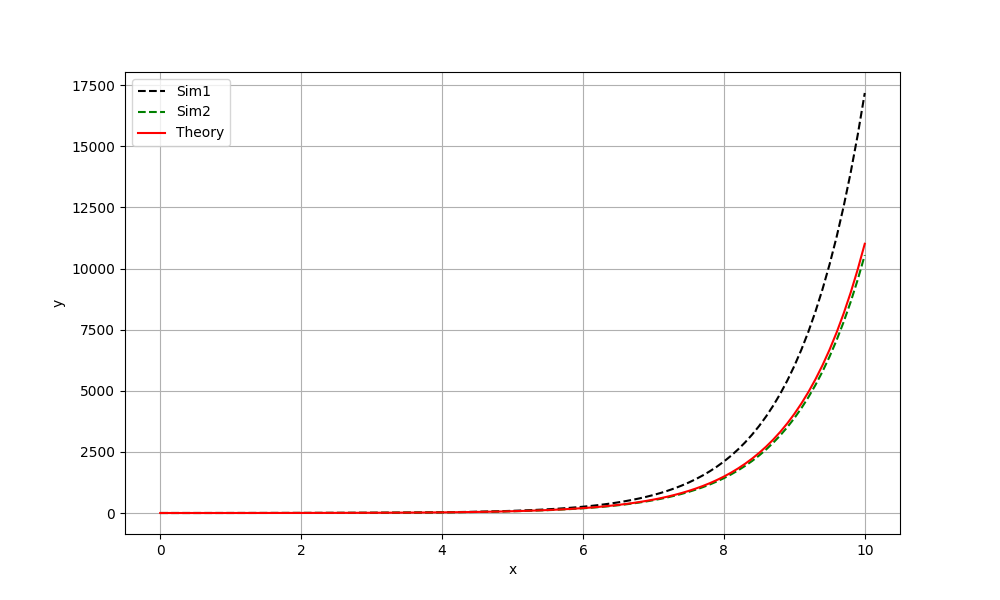
\includegraphics[width=0.8\columnwidth]{figs/fig.png}
    \caption{Comparison between the Theoritical solution and Computational solutions, Red is theory, Black line is derived from difference equation from Trapezoidal method, while Green line is from Z-transform while taking stepsize to be 0.1}
    \end{figure}   
\end{frame}
\end{document}

